\documentclass{report}
\usepackage[spanish]{babel}
\usepackage[utf8]{inputenc}
\usepackage{graphicx, longtable, float, titlesec, hyperref, enumitem, dingbat, soul, multicol, listings}
\usepackage[dvipsnames]{xcolor}
\usepackage[margin=2cm]{geometry}

% Cambia el color de los links
\hypersetup{
    hidelinks = true
}

% Python Code
\lstdefinestyle{Python}{
  commentstyle=\color{brown},
  keywordstyle=\color{violet},
  numberstyle=\tiny\color{gray},
  stringstyle=\color{purple},
  basicstyle=\ttfamily\footnotesize,
  breakatwhitespace=false,         
  breaklines=true,                 
  captionpos=b,                    
  keepspaces=true,                 
  numbers=left,                    
  numbersep=5pt,                  
  showspaces=false,                
  showstringspaces=false,
  showtabs=false,                  
  tabsize=2,
  literate={ñ}{{\~n}}1 {á}{{\'a}}1 {é}{{\'e}}1 {í}{{\'i}}1 {ó}{{\'o}}1 {ú}{{\'u}}1
}
\lstset{style=Python}

% Elimina la palabra "Capítulo" de los títulos de los capítulos
\titleformat{\chapter}[display]
  {\normalfont\bfseries}{}{0pt}{\Huge\thechapter.\space}

\titleformat{name=\chapter,numberless}[display]
  {\normalfont\bfseries}{}{0pt}{\Huge}

\titlespacing*{\chapter}{0pt}{-50pt}{20pt}

% Personalización del índice de listados
\renewcommand{\lstlistingname}{Código}  % Cambiar el nombre de "Listing" a "Código"
\renewcommand{\lstlistlistingname}{Índice de Códigos}

% Añade numeración a los subsubsections y los añade al índice
\setcounter{secnumdepth}{4}
\setcounter{tocdepth}{4}

\begin{document}
    \begin{titlepage}
        \centering
        
\includegraphics[width=0.6\textwidth]{./.img/logo.jpg}\\
        \vspace{1cm}
        \LARGE Técnicas de Inteligencia Artificial\\
        \vspace{0.5cm}
        \Large Ingeniería Informática de Gestión y Sistemas de Información\\
        \vspace{3cm}
        \Huge Practica 1\\
        \huge Problemas de Búsqueda\\
        \vspace{2.5cm}
        \Large Autor(es):\\
        \vspace{0.2cm}
        \large Xabier Gabiña\\
        \large Diego Montoya\\
        \vfill
        \today
    \end{titlepage}
    \tableofcontents
    \listoffigures
    \lstlistoflistings
    \chapter{Introducción}
      {
        En el marco de la asignatura de Técnicas de Inteligencia Artificial, se nos ha propuesto implementar y analizar diversos algoritmos de búsqueda aplicados al contexto de un proyecto académico desarrollado por la Universidad de Berkeley, basado en el clásico juego Pacman. El objetivo principal de esta práctica es profundizar en el funcionamiento de diferentes estrategias de búsqueda, estudiando su eficiencia y comportamiento en diferentes escenarios.\\

        Los algoritmos de búsqueda son fundamentales en el campo de la inteligencia artificial, ya que permiten encontrar soluciones óptimas o satisfactorias en problemas complejos. En esta práctica, nos enfocaremos en tres tipos de algoritmos de búsqueda no informados: Depth First Search (DFS), Breadth First Search (BFS) y Uniform Cost Search (UCS). Además, exploraremos un algoritmo de búsqueda informado: A*. Cada uno de estos algoritmos tiene sus propias características y aplicaciones, y su estudio nos permitirá comprender mejor sus ventajas y limitaciones.\\

        A lo largo de este documento, se presentarán las implementaciones de cada uno de estos algoritmos, junto con una descripción detallada de su funcionamiento y análisis de su rendimiento. Se incluirán ejemplos prácticos y se discutirán los resultados obtenidos en diferentes escenarios de búsqueda. El objetivo es proporcionar una visión completa y comprensiva de cómo estos algoritmos pueden ser aplicados en la resolución de problemas de búsqueda en inteligencia artificial.\\
      }
    \chapter{Ejercicios}
      \section{DFS - Depth First Search}
        \subsection*{Descripción}
          \paragraph*{}{
            DFS o Depth First Search es un algoritmo de búsqueda no informado,no emplea información adicional que no sean los nodos y sus arcos, este algoritmoque se basa en la exploración de todos los nodos de un grafo siguiendo una rama hasta llegar a un nodo hoja, para después retroceder y explorar otra rama.\\
            
            Este algoritmo se implementa mediante una pila, en la que se van almacenando los nodos a visitar.\\
            La pila es una estructura de datos de tipo LIFO (Last in First Out). La cual nos sirve para poder explorar por profundidad el árbol, gracias a l apila podemos recordar los nodos que deben de visitarse.\\
            
            Su coste en tiempo es de O(b\textsuperscript{m}), donde b es el factor de ramificación y m es la profundidad máxima del árbol.\\
            Su coste en espacio es de O(bm), donde b es el factor de ramificación y m es la profundidad máxima del árbol.\\
          }
        \subsection*{Primera implementación}
          \begin{lstlisting}[language=Python, caption=Implementación inicial del DFS]
  def depthFirstSearch(problem):
    """
    Implementación del algoritmo de búsqueda en profundidad.

    Args:
        problem (SearchProblem): Problema de búsqueda
    Returns:
        list: Lista de acciones para llegar al objetivo
    """
      stack = [problem] # Pila para almacenar los nodos a visitar
      visited = set()     # Conjunto para almacenar los nodos visitados
      path = []           # Lista para almacenar el camino al nodo objetivo

      while stack:    # Mientras haya elementos en el stack
          nodo_actual = stack.pop()   # Sacar el último elemento de la pila
          if nodo_actual in visited:  # Si el nodo actual ya ha sido visitado
              continue
          visited.add(nodo_actual)   # Marcar el nodo actual como visitado
          path.append(nodo_actual.contenido)  # Añadir el nodo actual al camino
          if nodo_actual.isGoalState():  # Si el nodo actual es el objetivo
              return path
          for hijo in reversed(nodo_actual.getSuccesor()): # Añadir los hijos del nodo actual a la pila
              stack.append(hijo)
          \end{lstlisting}
        \clearpage\subsection*{Implementación Final}
          \begin{lstlisting}[language=Python, caption=Implementación final del DFS]
  def depthFirstSearch(problem):
    """
    Implementación del algoritmo de búsqueda en profundidad.

    Args:
        problem (SearchProblem): Problema de búsqueda
    Returns:
        list: Lista de acciones para llegar al objetivo
    """
    stack = util.Stack()  # Añadir el nodo inicial a la pila
    stack.push([problem.getStartState(), []])
    visited = set()  # Conjunto para almacenar los nodos visitados

    while not stack.isEmpty():  # Mientras haya elementos en el stack
        nodo_actual = stack.pop()  # Sacar el último elemento de la pila
        if problem.isGoalState(nodo_actual[0]):  # Si el nodo actual es el objetivo
            return nodo_actual[1]  # Devolver el camino
        if nodo_actual[0] not in visited:
            visited.add(nodo_actual[0])
            for estado, accion, costo in reversed(problem.getSuccessors(nodo_actual[0])): 
                camino = nodo_actual[1] + [accion]
                stack.push([estado, camino])
          \end{lstlisting}
        \subsection*{Comentarios}
          \paragraph*{}{
            En la implementación inicial del algoritmo DFS, la implementacion de la lista del path es incorrecta por dos motivos. 
            El primero, es que se añade el nodo actual al path y no la accion que se ha de tomar para llegar a la meta.
            La segunda, es que se añaden todos los nodos visitados al path en orden de visita lo que hace que si llegamos a una hoja final se crea un salto en el path que seria imposible de realizar.\\
            Ambos problemas se han solucionado en la implementación final del algoritmo DFS.\\
          }
      \clearpage\section{BFS - Breadth First Search}
        \subsection*{Descripción}
          \paragraph*{}{
            BFS o Breadth First Search es un algoritmo de búsqueda no informado que se basa en la exploración de todos los nodos de un grafo nivel por nivel. Este algoritmo se implementa mediante una cola en la que se van almacenando los nodos que se deben visitar, manteniendo un orden de llegada basado en los niveles.\\ 
            Su coste en tiempo es de O(b\textsuperscript{d}), donde b es el factor de ramificación y d es la profundidad del nodo más cercano del árbol y su coste en espacio es de O(b\textsuperscript{d}), ya que debe almacenar todos los nodos del nivel actual antes de pasar al siguiente.\\
          }
        \subsection*{Implementación Final}
          \begin{lstlisting}[language=Python, caption=Implementación final del BFS]
  def breadthFirstSearch(problem):
    """
    Implementacion del algoritmo de busqueda en anchura.

    Args:
        problem (SearchProblem): Problema de busqueda
    Returns:
        list: Lista de acciones para llegar al objetivo
    """
    queue = util.Queue()  # Añadir el nodo inicial a la cola
    queue.push([problem.getStartState(), []])
    visited = set()     # Conjunto para almacenar los nodos visitados

    while not queue.isEmpty():    # Mientras haya elementos en la cola
        nodo_actual = queue.pop()   # Sacar el primer elemento de la cola
        if problem.isGoalState(nodo_actual[0]):  # Si el nodo actual es el objetivo
            return nodo_actual[1]  # Devolver el camino
        if nodo_actual[0] not in visited:
            visited.add(nodo_actual[0])
            for estado, accion, costo in problem.getSuccessors(nodo_actual[0]): # Añadir los hijos del nodo actual a la cola
                camino = nodo_actual[1] + [accion]
                queue.push([estado, camino])
          \end{lstlisting}
        \subsection*{Comentarios}
          \paragraph*{}{
            Este algoritmo ha tenido una sencilla implementación, ya que las dos unicas diferencias con el caso anterior es el cambio de la pila por una cola y que al añadir los nodos no es necesario hacerlo en el orden inverso ya que la cola mantiene el orden de llegada.\\
          }
      \clearpage\section{UCS - Uniform Cost Search}
        \subsection*{Descripción}
          \paragraph*{}{
            UCS o Uniform Cost Search es un algoritmo de búsqueda no informada que expande los nodos en función del costo acumulado. En contrario al BFS que prioriza la profundidad de los nodos el UCS utiliza la cola de prioridad para ordenar los nodos dependiendo su costo acumulado y expande primero el nodo con menor costo, obteniendo así una solución óptima en términos de costo.\\  
            El coste en tiempo del UCS es de \( O(b^{1 +\frac{ C^*}{\varepsilon}}) \), donde b es el factor de ramificación, C* es el costo de la solución óptima y \( \varepsilon \)  es el menor costo de transición entre nodos. Su coste de espacio es así mismo \( O(b^{1 +\frac{ C^*}{\varepsilon}}) \) ya que debe de almacenar todos los nodos en la cola de prioridad hasta encontrar la solución óptima \\
          }
        \subsection*{Implementación Final}
          \begin{lstlisting}[language=Python, caption=Implementación final del UCS]
def uniformCostSearch(problem):
  """
  Implementacion del algoritmo de busqueda de coste uniforme.

  Args:
      problem (SearchProblem): Problema de busqueda
  Returns:
      list: Lista de acciones para llegar al objetivo
  """
  queue = util.PriorityQueue()  # Añadir el nodo inicial a el heap
  queue.push([problem.getStartState(), [], 0], 0)
  visited = set()     # Conjunto para almacenar los nodos visitados

  while not queue.isEmpty():    # Mientras haya elementos en el stack
      nodo_actual = queue.pop()   # Sacar el último elemento de la pila
      if problem.isGoalState(nodo_actual[0]):  # Si el nodo actual es el objetivo
          return nodo_actual[1]  # Devolver el camino
      if nodo_actual[0] not in visited:
          visited.add(nodo_actual[0])
          for estado, accion, costo in problem.getSuccessors(nodo_actual[0]): # Añadir los hijos del nodo actual a la pila
              camino = nodo_actual[1] + [accion]
              queue.push([estado, camino, nodo_actual[2] + costo], nodo_actual[2] + costo)
          \end{lstlisting}
        \subsection*{Comentarios}
          \paragraph*{}{
            Al igual que en el caso anterior, en este, solo hemos necesitado hacer dos cambios.
            El primero es que la cola pasa a ser una cola de prioridad y ligado a esto el metodo push de la misma requiere de un segundo argumento que es el valor de prioridad.
          }
      \clearpage\section{A* Search}
        \subsection*{Descripción}
          \paragraph*{}{
            El A* es un algoritmo de búsqueda informada que utiliza las ventajas del UCS y Greedy Best-First Search, utilizando una función heurística para guiar la búsqueda hacia el objetivo de una manera más eficiente. A* expande los nodos en mediante una función de costo total. Donde f(n) = g(n) + h(n), g(n) siendo el costo acumulado desde el nodo inicial hasta n y h(n) es una estimación heurística del costo n hasta el objetivo. Este algoritmo se implementa mediante una cola de prioridad , donde los nodos se ordenan según su valor f(n) y se expande primero el nodo con menor valor f(n).\\
            Su coste en tiempo es de O(b\textsuperscript{d}), donde b es el factor de ramificación y d es la profundidad de la solución óptima, sin embargo el tiempo puede reducirse si la heurística es eficiente. Así mismo su coste de espacio es de  O(b\textsuperscript{d}), ya que se debe de almacenar todos los nodos generados en la cola de prioridad para asegurar la solución óptima.
          }
        \subsection*{Implementación Final}
          \begin{lstlisting}[language=Python, caption=Implementación final del A*]
def manhattanHeuristic(state, problem):
  """
  Heuristica de Manhattan.
  
  Args:
      state (tuple): Coordenadas del estado
      problem (SearchProblem): Problema de busqueda
  Returns:
      int: Distancia de Manhattan al objetivo
  """
  return util.manhattanDistance(state, problem.goal)

def aStarSearch(problem, heuristic=nullHeuristic):
  """
  Implementacion del algoritmo de busqueda A*.

  Args:
      problem (SearchProblem): Problema de busqueda
      heuristic (function): Heuristica para el problema
  Returns:
      list: Lista de acciones para llegar al objetivo
  """
  queue = util.PriorityQueue()  # Añadir el nodo inicial a el heap
  queue.push([problem.getStartState(), [], 0], 0)
  visited = set()     # Conjunto para almacenar los nodos visitados

  while not queue.isEmpty():    # Mientras haya elementos en el stack
      nodo_actual = queue.pop()   # Sacar el último elemento de la pila
      if problem.isGoalState(nodo_actual[0]):  # Si el nodo actual es el objetivo
          return nodo_actual[1]  # Devolver el camino
      if nodo_actual[0] not in visited:
          visited.add(nodo_actual[0])
          for estado, accion, costo in problem.getSuccessors(nodo_actual[0]): # Añadir los hijos del nodo actual a la pila
              camino = nodo_actual[1] + [accion]
              queue.push([estado, camino, nodo_actual[2] + costo], nodo_actual[2] + costo + heuristic(estado, problem))        
          \end{lstlisting}
        \subsection*{Comentarios}
          \paragraph*{}{
            En este caso, la implementación del A* es muy similar a la del UCS, con la única diferencia de que se suma la heurística al valor de prioridad de la cola de prioridad.\\
            El euristico utilizado en este caso es la distancia de Manhattan, que es la suma de las distancias horizontales y verticales entre dos puntos. Unicamente se ha tenido que añadir la función manhattanHeuristic que calcula la distancia de Manhattan entre dos puntos del archivo util.py.\\
          }
      \clearpage\section{Corners Problem: Representación}
        \subsection*{Descripción}
          \paragraph*{}{
            En este problema, Pacman debe visitar las cuatro esquinas de un laberinto antes de que se considere que ha alcanzado el objetivo. El problema se define mediante un estado inicial, un estado objetivo y una serie de acciones que Pacman puede realizar para moverse por el laberinto.\\
            Para representar este problema, se ha definido una clase CornersProblem que hereda de la clase SearchProblem. Esta clase almacena la información del laberinto, la posición inicial de Pacman y las esquinas que deben ser visitadas. Además, se definen los métodos necesarios para obtener el estado inicial, comprobar si un estado es objetivo y obtener los sucesores de un estado dado.\\
          }
        \subsection*{Primera implementación}
          \begin{lstlisting}[language=Python, caption=Implementación inicial del problema de las esquinas]
class CornersProblem(search.SearchProblem):
  """
  This search problem finds paths through all four corners of a layout.

  You must select a suitable state space and successor function
  """

  def __init__(self, startingGameState):
      """
      Stores the walls, pacman's starting position and corners.
      """
      self.walls = startingGameState.getWalls()
      self.startingPosition = startingGameState.getPacmanPosition()
      top, right = self.walls.height - 2, self.walls.width - 2
      self.corners = ((1, 1), (1, top), (right, 1), (right, top))
      for corner in self.corners:
          if not startingGameState.hasFood(*corner):
              print('Warning: no food in corner ' + str(corner))
      self._expanded = 0  # DO NOT CHANGE; Number of search nodes expanded
      # Please add any code here which you would like to use
      # in initializing the problem
              
  def getStartState(self):
      return self.startingPosition

  def isGoalState(self, state):
      """
      Returns whether this search state is a goal state of the problem.
      """
      if state in self.corners:
          self.explored.add(state)
      if len(self.explored) == 4:
          return True
      return False

  def getSuccessors(self, state):
      """
      Returns successor states, the actions they require, and a cost of 1.

        As noted in search.py:
          For a given state, this should return a list of triples, (successor,
          action, stepCost), where 'successor' is a successor to the current
          state, 'action' is the action required to get there, and 'stepCost'
          is the incremental cost of expanding to that successor
      """

      successors = []
      for action in [Directions.NORTH, Directions.SOUTH, Directions.EAST, Directions.WEST]:
          x, y = state
          dx, dy = Actions.directionToVector(action)
          nextx, nexty = int(x + dx), int(y + dy)
          if not self.walls[nextx][nexty]:
              nextState = (nextx, nexty)
              cost = self.costFn(nextState)
              successors.append((nextState, action, cost))

      self._expanded += 1  # DO NOT CHANGE
      return successors

  def getCostOfActions(self, actions):
      """
      Returns the cost of a particular sequence of actions.  If those actions
      include an illegal move, return 999999.  This is implemented for you.
      """
      if actions is None: return 999999
      x, y = self.startingPosition
      for action in actions:
          dx, dy = Actions.directionToVector(action)
          x, y = int(x + dx), int(y + dy)
          if self.walls[x][y]: return 999999
      return len(actions)
          \end{lstlisting}
        \subsection*{Implementación Final}
          \begin{lstlisting}[language=Python, caption=Implementación final del problema de las esquinas]
class CornersProblem(search.SearchProblem):
  """
  This search problem finds paths through all four corners of a layout.

  You must select a suitable state space and successor function
  """

  def __init__(self, startingGameState):
      """
      Stores the walls, pacman's starting position and corners.
      """
      self.walls = startingGameState.getWalls()
      self.startingPosition = startingGameState.getPacmanPosition()
      top, right = self.walls.height - 2, self.walls.width - 2
      self.corners = ((1, 1), (1, top), (right, 1), (right, top))
      for corner in self.corners:
          if not startingGameState.hasFood(*corner):
              print('Warning: no food in corner ' + str(corner))
      self._expanded = 0  # DO NOT CHANGE; Number of search nodes expanded
      # Please add any code here which you would like to use
      # in initializing the problem
              
  def getStartState(self):
      """
      Returns the start state, including the initial position and the visited corners.
      """
      # The start state now includes an empty set of visited corners
      return (self.startingPosition, ())

  def isGoalState(self, state):
      """
      Returns whether this search state is a goal state of the problem.
      """
      # Unpack the state
      position, visitedCorners = state

      # Check if we have visited all four corners
      return len(visitedCorners) == 4

  def getSuccessors(self, state):
      """
      Returns successor states, the actions they require, and a cost of 1.
      """
      successors = []
      # Unpack the current state
      currentPosition, visitedCorners = state

      for action in [Directions.NORTH, Directions.SOUTH, Directions.EAST, Directions.WEST]:
          x, y = currentPosition
          dx, dy = Actions.directionToVector(action)
          nextx, nexty = int(x + dx), int(y + dy)

          # Check if the next position is a wall
          if not self.walls[nextx][nexty]:
              nextPosition = (nextx, nexty)
              # Check if we have reached a new corner
              newVisitedCorners = list(visitedCorners)
              if nextPosition in self.corners and nextPosition not in visitedCorners:
                  newVisitedCorners.append(nextPosition)

              # Create a new state with updated corner list
              nextState = (nextPosition, tuple(newVisitedCorners))
              cost = 1  # Step cost is always 1
              successors.append((nextState, action, cost))

      self._expanded += 1  # DO NOT CHANGE
      return successors

  def getCostOfActions(self, actions):
      """
      Returns the cost of a particular sequence of actions.  If those actions
      include an illegal move, return 999999.  This is implemented for you.
      """
      if actions is None: return 999999
      x, y = self.startingPosition
      for action in actions:
          dx, dy = Actions.directionToVector(action)
          x, y = int(x + dx), int(y + dy)
          if self.walls[x][y]: return 999999
      return len(actions)        
          \end{lstlisting}
        \subsection*{Comentarios}
          \paragraph*{}{
            El problema que hemos tenido en este ejercicio ha sido la definición del estado inicial. La primera aproximacion que se nos ocurrio fue la de eliminar los corners ya visitados de la definición del problema pero esto parecia generar conflicto por lo que decidimos añadir una tupla con los corners visitados al estado inicial.
            De esta forma ya tenemos una representación del estado inicial que incluye la posición de pacman y las esquinas visitadas y podemos implementar el metodo isGoalState de forma efectiva.
            }
          \begin{figure}[H]
            \centering
            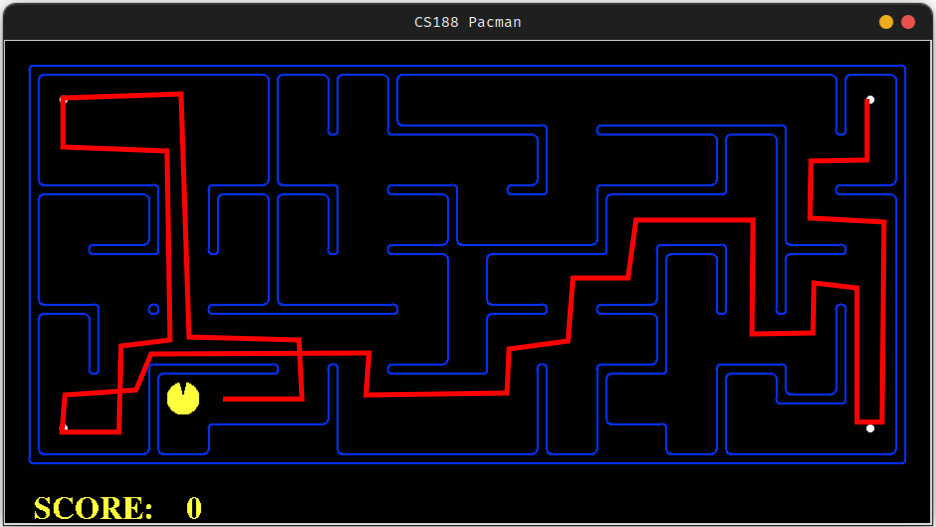
\includegraphics[width=0.7\textwidth]{.img/2.5-6.1.png}
            \caption{CornersProblem: Representación}
          \end{figure}
          \paragraph*{}{
            Con esta implementacion el pacman es capaz de recorrer todas las esquinas del laberinto.
          }
      \clearpage\section{Corners Problem: Heurística}
        \subsection*{Descripción}
          \paragraph*{}{
            En este problema, se nos pide implementar una heurística para el problema de las esquinas, que permita calcular una estimación del coste mínimo para visitar todas las esquinas restantes. La heurística debe ser admisible y consistente, es decir, no puede sobreestimar el coste real de llegar a la meta y debe ser siempre menor o igual al coste real.\\
            Para este problema, hemos implementado una heurística basada en la distancia de Manhattan, que calcula la distancia mínima entre la posición actual de Pacman y la esquina más cercana que aún no ha sido visitada. Esta heurística es admisible y consistente, ya que siempre subestima el coste real de recorrer todas las esquinas y es siempre menor o igual al coste real.\\
          }
        \subsection*{Primera implementación}
          \begin{lstlisting}[language=Python, caption=Implementación inicial de la heurística del problema de las esquinas]
def cornersHeuristic(state, problem):
  """
  A heuristic for the CornersProblem that you defined.

    state:   The current search state
              (a data structure you chose in your search problem)

    problem: The CornersProblem instance for this layout.

  This function should always return a number that is a lower bound on the
  shortest path from the state to a goal of the problem; i.e.  it should be
  admissible (as well as consistent).
  """
  currentPosition, visitedCorners = state
  corners = problem.corners

  # Identificar las esquinas que aún no han sido visitadas
  unvisitedCorners = [corner for corner in corners if corner not in visitedCorners]

  # Calcular la distancia mínima utilizando la distancia Manhattan
  current = currentPosition
  while unvisitedCorners:
    distances = [(util.manhattanDistance(current, corner), corner) for corner in unvisitedCorners]
    minDistance, closestCorner = min(distances)

    heuristic = minDistance
    current = closestCorner
    unvisitedCorners.remove(closestCorner)

  return heuristic
          \end{lstlisting}
        \subsection*{Implementación Final}
          \begin{lstlisting}[language=Python, caption=Implementación final de la heurística del problema de las esquinas]
def cornersHeuristic(state, problem):
  """
  A heuristic for the CornersProblem that you defined.

    state:   The current search state (currentPosition, visitedCorners)
    problem: The CornersProblem instance for this layout.
  """
  currentPosition, visitedCorners = state
  corners = problem.corners

  # Identificar las esquinas que aún no han sido visitadas
  unvisitedCorners = [corner for corner in corners if corner not in visitedCorners]

  # Calcular la distancia mínima utilizando la distancia Manhattan
  heuristic = 0
  current = currentPosition

  while unvisitedCorners:
      # Encontrar la esquina más cercana (distancia Manhattan)
      distances = [(util.manhattanDistance(current, corner), corner) for corner in unvisitedCorners]
      minDistance, closestCorner = min(distances)
      
      # Agregar la distancia mínima a la heurística y moverse a la siguiente esquina
      heuristic += minDistance
      current = closestCorner
      unvisitedCorners.remove(closestCorner)

  return heuristic        
          \end{lstlisting}
        \subsection*{Comentarios}
          \paragraph*{}{
            El principal error en la primera implementacion estaba en que no se estaba calculando la heuristica de forma correcta ya que se estaba usando como heuristica siempre la distancia minima entre la posicion actual y la esquina mas cercana cuando deberia estar dando el coste minimo de llegar a todas las esquinas restantes.
            Esto provocaba subestimar el costo real de recorrer todas las esquinas, ya que no se tienen en cuenta las distancias adicionales necesarias para visitar las otras esquinas.
          }
          \begin{figure}[H]
            \centering
            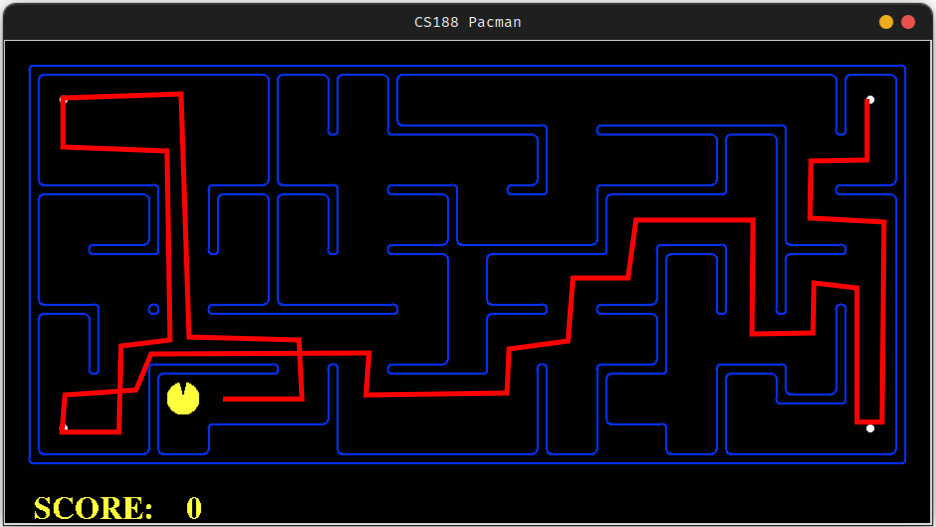
\includegraphics[width=0.7\textwidth]{.img/2.5-6.1.png}
            \caption{CornersProblem: Heuristic}
          \end{figure}
          \paragraph*{}{
            En este caso el resultado es igual al del ejercicio anterior pero al usar la euristica el numero de nodos que se han expandido es mucho menor.
          }
      \clearpage\section{Eating All The Dots: Heurística}
        \subsection*{Descripción}
          \paragraph*{}{
            En este problema, Pacman debe recoger todas las comidas del laberinto antes de que se considere que ha alcanzado el objetivo. El problema se define mediante un estado inicial, un estado objetivo y una serie de acciones que Pacman puede realizar para moverse por el laberinto.\\
            Para representar este problema, se ha definido una clase FoodSearchProblem que hereda de la clase SearchProblem. Esta clase almacena la información del laberinto, la posición inicial de Pacman y las comidas que deben ser recogidas. Además, se definen los métodos necesarios para obtener el estado inicial, comprobar si un estado es objetivo y obtener los sucesores de un estado dado.\\
          }
        \subsection*{Primera implementación}
          \begin{lstlisting}[language=Python, caption=Implementación inicial de la heurística del problema de las esquinas]
def foodHeuristic(state, problem):
  """
  A heuristic for the FoodSearchProblem.
  
  state: (pacmanPosition, foodGrid)
  problem: The FoodSearchProblem instance.
  """
  position, foodGrid = state

  # Convert foodGrid to a list of food positions
  foodList = foodGrid.asList()

  # Si no hay comida restante, la heurística es 0
  if not foodList:
      return 0

  # Calcular la distancia de laberinto a cada punto de comida desde la posición actual de Pacman
  distances = [mazeDistance(position, food, problem.startingGameState) for food in foodList]

  # La heurística es la distancia máxima a cualquier punto de comida
  return min(distances)
          \end{lstlisting}
        \subsection*{Implementación Final}
          \begin{lstlisting}[language=Python, caption=Implementación final de la heurística del problema de las esquinas]
def foodHeuristic(state, problem):
  """
  A heuristic for the FoodSearchProblem.
  
  state: (pacmanPosition, foodGrid)
  problem: The FoodSearchProblem instance.
  """
  position, foodGrid = state

  # Convert foodGrid to a list of food positions
  foodList = foodGrid.asList()

  # Si no hay comida restante, la heurística es 0
  if not foodList:
      return 0

  # Calcular la distancia de laberinto a cada punto de comida desde la posición actual de Pacman
  distances = [mazeDistance(position, food, problem.startingGameState) for food in foodList]

  # La heurística es la distancia máxima a cualquier punto de comida
  return max(distances)
          \end{lstlisting}
        \subsection*{Comentarios}
          \paragraph*{}{
            El problema en la primera implementación era que se estaba calculando la heurística como la distancia mínima a cualquier punto de comida, lo que subestima el costo real de recorrer todos los puntos de comida y provoca que se elijan caminos suboptimos al no tener en cuenta las comidas más lejanas.\\
          }
          \begin{figure}[H]
            \centering
            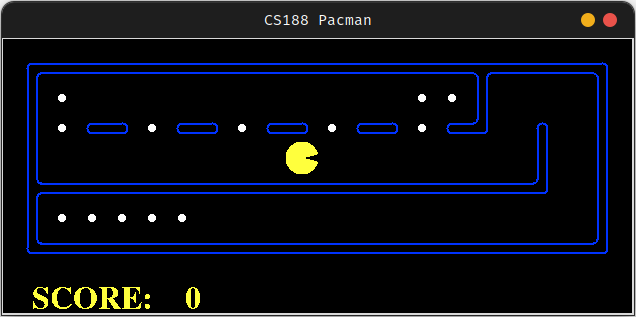
\includegraphics[width=0.7\textwidth]{.img/2.7.1.png}
            \caption{FoodSearchProblem inicio}
          \end{figure}
          \begin{figure}[H]
            \centering
            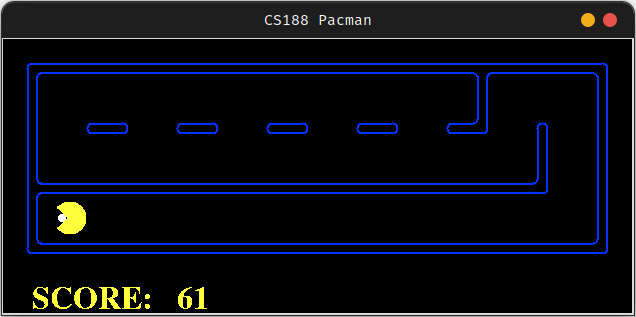
\includegraphics[width=0.7\textwidth]{.img/2.7.2.png}
            \caption{FoodSearchProblem final}
          \end{figure}
          \paragraph*{}{
            Una vez solventado el problema, el pacman es capaz de encontrar el camino más corto para recoger todas las comidas del laberinto.\\
          }
      \clearpage\section{Suboptimal Search}
        \subsection*{Descripción}
          \paragraph*{}{
            En este problema, se nos pide implementar un agente de búsqueda que encuentre un camino subóptimo para recoger todas las comidas del laberinto. El agente debe utilizar una secuencia de búsquedas para encontrar el camino más corto hacia el punto de comida más cercano y repetir este proceso hasta que todas las comidas hayan sido recogidas.\\
            Para implementar este agente, hemos definido una clase ClosestDotSearchAgent que hereda de la clase SearchAgent. Esta clase almacena las acciones que tomará Pacman para recoger todas las comidas y utiliza una secuencia de búsquedas para encontrar el camino más corto hacia el punto de comida más cercano.\\
          }
        \subsection*{Implementación Final}
          \begin{lstlisting}[language=Python, caption=Implementación final del problema de las esquinas]
class ClosestDotSearchAgent(SearchAgent):
  """Search for all food using a sequence of searches"""

  def registerInitialState(self, state):
      """
      El agente registra el estado inicial y sigue buscando el punto de comida más cercano
      hasta que todos los puntos de comida hayan sido consumidos.
      """
      self.actions = []  # Almacena las acciones que tomará Pacman
      currentState = state

      # Repite mientras haya puntos de comida restantes
      while currentState.getFood().count() > 0:
          # Encuentra el camino hacia el punto de comida más cercano
          nextPathSegment = self.findPathToClosestDot(currentState)
          
          # Añade estas acciones al plan del agente
          self.actions += nextPathSegment

          # Asegura que todas las acciones sean válidas
          for action in nextPathSegment:
              legal = currentState.getLegalActions()
              if action not in legal:
                  raise Exception(f'findPathToClosestDot returned an illegal move: {action}!\n{currentState}')
              
              # Genera el siguiente estado sucesor para Pacman
              currentState = currentState.generateSuccessor(0, action)

      self.actionIndex = 0
      print(f'Path found with cost {len(self.actions)}.')

  def findPathToClosestDot(self, gameState):
      """
      Devuelve una lista de acciones que llevan al punto de comida más cercano, comenzando desde el estado actual del juego.
      """
      # Define un problema de búsqueda para cualquier alimento disponible
      problem = AnyFoodSearchProblem(gameState)

      # Utiliza el algoritmo de búsqueda (BFS en este caso) para encontrar el camino más corto hacia el punto de comida más cercano
      from search import breadthFirstSearch
      return breadthFirstSearch(problem)


class AnyFoodSearchProblem(PositionSearchProblem):
  """
  Un problema de búsqueda para encontrar un camino a cualquier punto de comida.
  Este problema es similar a PositionSearchProblem, pero con un objetivo distinto: cualquier punto de comida.
  """

  def __init__(self, gameState):
      """Almacena la información del estado de juego para su uso posterior."""
      # Almacena los alimentos del estado de juego actual
      self.food = gameState.getFood()

      # Llama al constructor de PositionSearchProblem
      super().__init__(gameState)
      self.walls = gameState.getWalls()
      self.startState = gameState.getPacmanPosition()
      self.costFn = lambda x: 1  # El costo de cada acción es 1

      # Variables de seguimiento (no es necesario modificar)
      self._visited, self._visitedlist, self._expanded = {}, [], 0

  def isGoalState(self, state):
      """
      Devuelve si el estado actual (la posición de Pacman) es un estado objetivo.
      El estado es un objetivo si contiene un punto de comida.
      """
      x, y = state
      # El estado es objetivo si hay comida en la posición actual de Pacman
      return self.food[x][y]
          \end{lstlisting}
        \subsection*{Comentarios}
          \paragraph*{}{
            En este caso, la implementacion del agente ClosestDotSearchAgent es muy sencilla, ya que simplemente se encarga de buscar el camino más corto hacia el punto de comida más cercano y añadirlo a la lista de acciones que tomará Pacman.
            Para ello reciclamos la implementacion del algoritmo BFS que ya teniamos implementado ya que es el algoritmo más adecuado para encontrar el camino más corto en este caso.\\

            De esta forma, el agente ClosestDotSearchAgent se encarga de encontrar el camino más corto hacia el punto de comida más cercano y repetir este proceso hasta que todas las comidas hayan sido recogidas.\\
          }
          \begin{figure}[H]
            \centering
            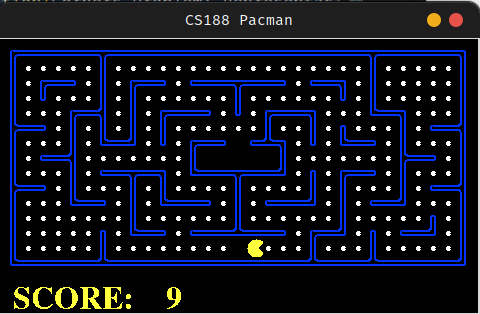
\includegraphics[width=0.7\textwidth]{.img/2.8.1.png}
            \caption{ClosestDotSearchAgent inicio}
          \end{figure}
          \begin{figure}[H]
            \centering
            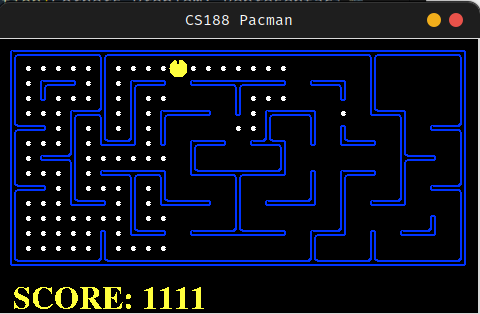
\includegraphics[width=0.7\textwidth]{.img/2.8.2.png}
            \caption{ClosestDotSearchAgent intermedio}
          \end{figure}
          \begin{figure}[H]
            \centering
            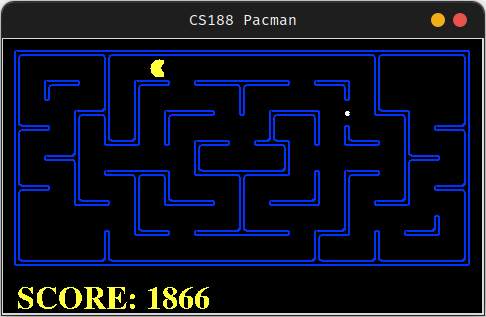
\includegraphics[width=0.7\textwidth]{.img/2.8.3.png}
            \caption{ClosestDotSearchAgent final}
          \end{figure}
          \paragraph*{}
          {
            Como podemos ver en la ejecucion del agente, al comer simplemente teniendo en cuenta el punto de comida más cercano, no siempre se consigue el camino más corto para recoger todas las comidas.\\
          }
    \chapter{Resultados}
      \section{Casos de pruebas}
        \subsection{DFS}
          \begin{lstlisting}[language=Python, caption=Prueba DFS]
python pacman.py -l tinyMaze -p SearchAgent -a fn=tinyMazeSearch
[SearchAgent] using function tinyMazeSearch
[SearchAgent] using problem type PositionSearchProblem
Path found with total cost of 8 in 0.0 seconds
Search nodes expanded: 0
Pacman emerges victorious! Score: 502
Average Score: 502.0
Scores:        502.0
Win Rate:      1/1 (1.00)
Record:        Win

python pacman.py -l tinyMaze -p SearchAgent
[SearchAgent] using function depthFirstSearch
[SearchAgent] using problem type PositionSearchProblem
Path found with total cost of 8 in 0.0 seconds
Search nodes expanded: 15
Pacman emerges victorious! Score: 502
Average Score: 502.0
Scores:        502.0
Win Rate:      1/1 (1.00)
Record:        Win

python pacman.py -l mediumMaze -p SearchAgent
[SearchAgent] using function depthFirstSearch
[SearchAgent] using problem type PositionSearchProblem
Path found with total cost of 246 in 0.0 seconds
Search nodes expanded: 269
Pacman emerges victorious! Score: 264
Average Score: 264.0
Scores:        264.0
Win Rate:      1/1 (1.00)
Record:        Win

python pacman.py -l bigMaze -z .5 -p SearchAgent
[SearchAgent] using function depthFirstSearch
[SearchAgent] using problem type PositionSearchProblem
Path found with total cost of 210 in 0.0 seconds
Search nodes expanded: 466
Pacman emerges victorious! Score: 300
Average Score: 300.0
Scores:        300.0
Win Rate:      1/1 (1.00)
Record:        Win
          \end{lstlisting}
        \clearpage\subsection{BFS}
          \begin{lstlisting}[language=Python, caption=Prueba BFS]
python pacman.py -l mediumMaze -p SearchAgent -a fn=bfs
[SearchAgent] using function bfs
[SearchAgent] using problem type PositionSearchProblem
Path found with total cost of 68 in 0.0 seconds
Search nodes expanded: 269
Pacman emerges victorious! Score: 442
Average Score: 442.0
Scores:        442.0
Win Rate:      1/1 (1.00)
Record:        Win

python pacman.py -l bigMaze -z .5 -p SearchAgent -a fn=bfs
[SearchAgent] using function bfs
[SearchAgent] using problem type PositionSearchProblem
Path found with total cost of 210 in 0.0 seconds
Search nodes expanded: 620
Pacman emerges victorious! Score: 300
Average Score: 300.0
Scores:        300.0
Win Rate:      1/1 (1.00)
Record:        Win

python eightpuzzle.py
A random puzzle:
-------------
| 2 |   | 5 |
-------------
| 3 | 4 | 1 |
-------------
| 6 | 7 | 8 |
-------------
BFS found a path of 9 moves: ['left', 'down', 'right', 'right', 'up', 'left', 'down', 'left', 'up']
After 1 move: left
-------------
|   | 2 | 5 |
-------------
| 3 | 4 | 1 |
-------------
| 6 | 7 | 8 |
-------------
Press return for the next state...
After 2 moves: down
-------------
| 3 | 2 | 5 |
-------------
|   | 4 | 1 |
-------------
| 6 | 7 | 8 |
-------------
Press return for the next state...
After 3 moves: right
-------------
| 3 | 2 | 5 |
-------------
| 4 |   | 1 |
-------------
| 6 | 7 | 8 |
-------------
Press return for the next state...
After 4 moves: right
-------------
| 3 | 2 | 5 |
-------------
| 4 | 1 |   |
-------------
| 6 | 7 | 8 |
-------------
Press return for the next state...
After 5 moves: up
-------------
| 3 | 2 |   |
-------------
| 4 | 1 | 5 |
-------------
| 6 | 7 | 8 |
-------------
Press return for the next state...
After 6 moves: left
-------------
| 3 |   | 2 |
-------------
| 4 | 1 | 5 |
-------------
| 6 | 7 | 8 |
-------------
Press return for the next state...
After 7 moves: down
-------------
| 3 | 1 | 2 |
-------------
| 4 |   | 5 |
-------------
| 6 | 7 | 8 |
-------------
Press return for the next state...
After 8 moves: left
-------------
| 3 | 1 | 2 |
-------------
|   | 4 | 5 |
-------------
| 6 | 7 | 8 |
-------------
Press return for the next state...
After 9 moves: up
-------------
|   | 1 | 2 |
-------------
| 3 | 4 | 5 |
-------------
| 6 | 7 | 8 |
-------------
Press return for the next state...
          \end{lstlisting}
        \clearpage\subsection{UCS}
          \begin{lstlisting}[language=Python, caption=Prueba UCS]
python pacman.py -l mediumMaze -p SearchAgent -a fn=ucs
[SearchAgent] using function ucs
[SearchAgent] using problem type PositionSearchProblem
Path found with total cost of 68 in 0.0 seconds
Search nodes expanded: 269
Pacman emerges victorious! Score: 442
Average Score: 442.0
Scores:        442.0
Win Rate:      1/1 (1.00)
Record:        Win

python pacman.py -l mediumDottedMaze -p StayEastSearchAgent
[SearchAgent] using function depthFirstSearch
[SearchAgent] using problem type PositionSearchProblem
Path found with total cost of 1.000976583804004 in 0.0 seconds
Search nodes expanded: 186
Pacman emerges victorious! Score: 646
Average Score: 646.0
Scores:        646.0
Win Rate:      1/1 (1.00)
Record:        Win

python pacman.py -l mediumScaryMaze -p StayWestSearchAgent
[SearchAgent] using function depthFirstSearch
[SearchAgent] using problem type PositionSearchProblem
Path found with total cost of 68719479864 in 0.0 seconds
Search nodes expanded: 108
Pacman emerges victorious! Score: 418
Average Score: 418.0
Scores:        418.0
Win Rate:      1/1 (1.00)
Record:        Win
          \end{lstlisting}
        \clearpage\subsection{A*}
          \begin{lstlisting}[language=Python, caption=Prueba A*]
python pacman.py -l bigMaze -z .5 -p SearchAgent -a fn=astar,heuristic=manhattanHeuristic
[SearchAgent] using function astar and heuristic manhattanHeuristic
[SearchAgent] using problem type PositionSearchProblem
Path found with total cost of 210 in 0.0 seconds
Search nodes expanded: 549
Pacman emerges victorious! Score: 300
Average Score: 300.0
Scores:        300.0
Win Rate:      1/1 (1.00)
Record:        Win
          \end{lstlisting}
        \clearpage\subsection{Corners Problem: Representación}
          \begin{lstlisting}[language=Python, caption=Prueba Representación Corners Problem]
python pacman.py -l tinyCorners -p SearchAgent -a fn=bfs,prob=CornersProblem
[SearchAgent] using function bfs
[SearchAgent] using problem type CornersProblem
Path found with total cost of 28 in 0.0 seconds
Search nodes expanded: 435
Pacman emerges victorious! Score: 512
Average Score: 512.0
Scores:        512.0
Win Rate:      1/1 (1.00)
Record:        Win

python pacman.py -l mediumCorners -p SearchAgent -a fn=bfs,prob=CornersProblem
[SearchAgent] using function bfs
[SearchAgent] using problem type CornersProblem
Path found with total cost of 106 in 0.0 seconds
Search nodes expanded: 2448
Pacman emerges victorious! Score: 434
Average Score: 434.0
Scores:        434.0
Win Rate:      1/1 (1.00)
Record:        Win
          \end{lstlisting}
        \clearpage\subsection{Corners Problem: Heurística}
          \begin{lstlisting}[language=Python, caption=Prueba Heurística Corners Problem]
python pacman.py -l mediumCorners -p AStarCornersAgent -z 0.5
[SearchAgent] using function depthFirstSearch
[SearchAgent] using problem type PositionSearchProblem
Path found with total cost of 106 in 0.0 seconds
Search nodes expanded: 901
Pacman emerges victorious! Score: 434
Average Score: 434.0
Scores:        434.0
Win Rate:      1/1 (1.00)
Record:        Win
          \end{lstlisting}
        \clearpage\subsection{Eating All The Dots}
          \begin{lstlisting}[language=Python, caption=Prueba Eating All The Dots]
python pacman.py -l testSearch -p AStarFoodSearchAgent
[SearchAgent] using function depthFirstSearch
[SearchAgent] using problem type PositionSearchProblem
Path found with total cost of 7 in 0.0 seconds
Search nodes expanded: 10
Pacman emerges victorious! Score: 513
Average Score: 513.0
Scores:        513.0
Win Rate:      1/1 (1.00)
Record:        Win

python pacman.py -l trickySearch -p AStarFoodSearchAgent
[SearchAgent] using function depthFirstSearch
[SearchAgent] using problem type PositionSearchProblem
Path found with total cost of 60 in 17.1 seconds
Search nodes expanded: 4137
Pacman emerges victorious! Score: 570
Average Score: 570.0
Scores:        570.0
Win Rate:      1/1 (1.00)
Record:        Win
          \end{lstlisting}
        \clearpage\subsection{Suboptimal Search}
          \begin{lstlisting}[language=Python, caption=Prueba Suboptimal Search]
python pacman.py -l bigSearch -p ClosestDotSearchAgent -z .5
[SearchAgent] using function depthFirstSearch
[SearchAgent] using problem type PositionSearchProblem
Warning: this does not look like a regular search maze
Path found with cost 350.
Pacman emerges victorious! Score: 2360
Average Score: 2360.0
Scores:        2360.0
Win Rate:      1/1 (1.00)
Record:        Win
          \end{lstlisting}
      \clearpage\section{Autograder}
          \begin{lstlisting}
Starting on 10-6 at 13:02:51

Question q1
===========

*** PASS: test_cases/q1/graph_backtrack.test
*** 	solution:		['1:A->C', '0:C->G']
*** 	expanded_states:	['A', 'B', 'C']
*** PASS: test_cases/q1/graph_bfs_vs_dfs.test
*** 	solution:		['0:A->B', '0:B->D', '0:D->G']
*** 	expanded_states:	['A', 'B', 'D']
*** PASS: test_cases/q1/graph_infinite.test
*** 	solution:		['0:A->B', '1:B->C', '1:C->G']
*** 	expanded_states:	['A', 'B', 'C']
*** PASS: test_cases/q1/graph_manypaths.test
*** 	solution:		['0:A->B1', '0:B1->C', '0:C->D', '0:D->E1', '0:E1->F', '0:F->G']
*** 	expanded_states:	['A', 'B1', 'C', 'D', 'E1', 'F']
*** PASS: test_cases/q1/pacman_1.test
*** 	pacman layout:		mediumMaze
*** 	solution length: 246
*** 	nodes expanded:		269

### Question q1: 3/3 ###


Question q2
===========

*** PASS: test_cases/q2/graph_backtrack.test
*** 	solution:		['1:A->C', '0:C->G']
*** 	expanded_states:	['A', 'B', 'C', 'D']
*** PASS: test_cases/q2/graph_bfs_vs_dfs.test
*** 	solution:		['1:A->G']
*** 	expanded_states:	['A', 'B']
*** PASS: test_cases/q2/graph_infinite.test
*** 	solution:		['0:A->B', '1:B->C', '1:C->G']
*** 	expanded_states:	['A', 'B', 'C']
*** PASS: test_cases/q2/graph_manypaths.test
*** 	solution:		['1:A->C', '0:C->D', '1:D->F', '0:F->G']
*** 	expanded_states:	['A', 'B1', 'C', 'B2', 'D', 'E1', 'F', 'E2']
*** PASS: test_cases/q2/pacman_1.test
*** 	pacman layout:		mediumMaze
*** 	solution length: 68
*** 	nodes expanded:		269

### Question q2: 3/3 ###


Question q3
===========

*** PASS: test_cases/q3/graph_backtrack.test
*** 	solution:		['1:A->C', '0:C->G']
*** 	expanded_states:	['A', 'B', 'C', 'D']
*** PASS: test_cases/q3/graph_bfs_vs_dfs.test
*** 	solution:		['1:A->G']
*** 	expanded_states:	['A', 'B']
*** PASS: test_cases/q3/graph_infinite.test
*** 	solution:		['0:A->B', '1:B->C', '1:C->G']
*** 	expanded_states:	['A', 'B', 'C']
*** PASS: test_cases/q3/graph_manypaths.test
*** 	solution:		['1:A->C', '0:C->D', '1:D->F', '0:F->G']
*** 	expanded_states:	['A', 'B1', 'C', 'B2', 'D', 'E1', 'F', 'E2']
*** PASS: test_cases/q3/ucs_0_graph.test
*** 	solution:		['Right', 'Down', 'Down']
*** 	expanded_states:	['A', 'B', 'D', 'C', 'G']
*** PASS: test_cases/q3/ucs_1_problemC.test
*** 	pacman layout:		mediumMaze
*** 	solution length: 68
*** 	nodes expanded:		269
*** PASS: test_cases/q3/ucs_2_problemE.test
*** 	pacman layout:		mediumMaze
*** 	solution length: 74
*** 	nodes expanded:		260
*** PASS: test_cases/q3/ucs_3_problemW.test
*** 	pacman layout:		mediumMaze
*** 	solution length: 152
*** 	nodes expanded:		173
*** PASS: test_cases/q3/ucs_4_testSearch.test
*** 	pacman layout:		testSearch
*** 	solution length: 7
*** 	nodes expanded:		14
*** PASS: test_cases/q3/ucs_5_goalAtDequeue.test
*** 	solution:		['1:A->B', '0:B->C', '0:C->G']
*** 	expanded_states:	['A', 'B', 'C']

### Question q3: 3/3 ###


Question q4
===========

*** PASS: test_cases/q4/astar_0.test
*** 	solution:		['Right', 'Down', 'Down']
*** 	expanded_states:	['A', 'B', 'D', 'C', 'G']
*** PASS: test_cases/q4/astar_1_graph_heuristic.test
*** 	solution:		['0', '0', '2']
*** 	expanded_states:	['S', 'A', 'D', 'C']
*** PASS: test_cases/q4/astar_2_manhattan.test
*** 	pacman layout:		mediumMaze
*** 	solution length: 68
*** 	nodes expanded:		221
*** PASS: test_cases/q4/astar_3_goalAtDequeue.test
*** 	solution:		['1:A->B', '0:B->C', '0:C->G']
*** 	expanded_states:	['A', 'B', 'C']
*** PASS: test_cases/q4/graph_backtrack.test
*** 	solution:		['1:A->C', '0:C->G']
*** 	expanded_states:	['A', 'B', 'C', 'D']
*** PASS: test_cases/q4/graph_manypaths.test
*** 	solution:		['1:A->C', '0:C->D', '1:D->F', '0:F->G']
*** 	expanded_states:	['A', 'B1', 'C', 'B2', 'D', 'E1', 'F', 'E2']

### Question q4: 3/3 ###


Question q5
===========

*** PASS: test_cases/q5/corner_tiny_corner.test
*** 	pacman layout:		tinyCorner
*** 	solution length:		28

### Question q5: 3/3 ###


Question q6
===========

*** PASS: heuristic value less than true cost at start state
*** PASS: heuristic value less than true cost at start state
*** PASS: heuristic value less than true cost at start state
path: ['North', 'East', 'East', 'East', 'East', 'North', 'North', 'West', 'West', 'West', 'West', 'North', 'North', 'North', 'North', 'North', 'North', 'North', 'North', 'West', 'West', 'West', 'West', 'South', 'South', 'East', 'East', 'East', 'East', 'South', 'South', 'South', 'South', 'South', 'South', 'West', 'West', 'South', 'South', 'South', 'West', 'West', 'East', 'East', 'North', 'North', 'North', 'East', 'East', 'East', 'East', 'East', 'East', 'East', 'East', 'South', 'South', 'East', 'East', 'East', 'East', 'East', 'North', 'North', 'East', 'East', 'North', 'North', 'East', 'East', 'North', 'North', 'East', 'East', 'East', 'East', 'South', 'South', 'South', 'South', 'East', 'East', 'North', 'North', 'East', 'East', 'South', 'South', 'South', 'South', 'South', 'North', 'North', 'North', 'North', 'North', 'North', 'North', 'West', 'West', 'North', 'North', 'East', 'East', 'North', 'North']
path length: 106
*** PASS: Heuristic resulted in expansion of 901 nodes

### Question q6: 3/3 ###


Question q7
===========

*** PASS: test_cases/q7/food_heuristic_1.test
*** PASS: test_cases/q7/food_heuristic_10.test
*** PASS: test_cases/q7/food_heuristic_11.test
*** PASS: test_cases/q7/food_heuristic_12.test
*** PASS: test_cases/q7/food_heuristic_13.test
*** PASS: test_cases/q7/food_heuristic_14.test
*** PASS: test_cases/q7/food_heuristic_15.test
*** PASS: test_cases/q7/food_heuristic_16.test
*** PASS: test_cases/q7/food_heuristic_17.test
*** PASS: test_cases/q7/food_heuristic_2.test
*** PASS: test_cases/q7/food_heuristic_3.test
*** PASS: test_cases/q7/food_heuristic_4.test
*** PASS: test_cases/q7/food_heuristic_5.test
*** PASS: test_cases/q7/food_heuristic_6.test
*** PASS: test_cases/q7/food_heuristic_7.test
*** PASS: test_cases/q7/food_heuristic_8.test
*** PASS: test_cases/q7/food_heuristic_9.test
*** PASS: test_cases/q7/food_heuristic_grade_tricky.test
*** 	expanded nodes: 4137
*** 	thresholds: [15000, 12000, 9000, 7000]

### Question q7: 5/4 ###


Question q8
===========

[SearchAgent] using function depthFirstSearch
[SearchAgent] using problem type PositionSearchProblem
Warning: this does not look like a regular search maze
*** PASS: test_cases/q8/closest_dot_1.test
*** 	pacman layout:		Test 1
*** 	solution length:		1
[SearchAgent] using function depthFirstSearch
[SearchAgent] using problem type PositionSearchProblem
Warning: this does not look like a regular search maze
*** PASS: test_cases/q8/closest_dot_10.test
*** 	pacman layout:		Test 10
*** 	solution length:		1
[SearchAgent] using function depthFirstSearch
[SearchAgent] using problem type PositionSearchProblem
Warning: this does not look like a regular search maze
*** PASS: test_cases/q8/closest_dot_11.test
*** 	pacman layout:		Test 11
*** 	solution length:		2
[SearchAgent] using function depthFirstSearch
[SearchAgent] using problem type PositionSearchProblem
Warning: this does not look like a regular search maze
*** PASS: test_cases/q8/closest_dot_12.test
*** 	pacman layout:		Test 12
*** 	solution length:		3
[SearchAgent] using function depthFirstSearch
[SearchAgent] using problem type PositionSearchProblem
Warning: this does not look like a regular search maze
*** PASS: test_cases/q8/closest_dot_13.test
*** 	pacman layout:		Test 13
*** 	solution length:		1
[SearchAgent] using function depthFirstSearch
[SearchAgent] using problem type PositionSearchProblem
Warning: this does not look like a regular search maze
*** PASS: test_cases/q8/closest_dot_2.test
*** 	pacman layout:		Test 2
*** 	solution length:		1
[SearchAgent] using function depthFirstSearch
[SearchAgent] using problem type PositionSearchProblem
Warning: this does not look like a regular search maze
*** PASS: test_cases/q8/closest_dot_3.test
*** 	pacman layout:		Test 3
*** 	solution length:		1
[SearchAgent] using function depthFirstSearch
[SearchAgent] using problem type PositionSearchProblem
Warning: this does not look like a regular search maze
*** PASS: test_cases/q8/closest_dot_4.test
*** 	pacman layout:		Test 4
*** 	solution length:		3
[SearchAgent] using function depthFirstSearch
[SearchAgent] using problem type PositionSearchProblem
Warning: this does not look like a regular search maze
*** PASS: test_cases/q8/closest_dot_5.test
*** 	pacman layout:		Test 5
*** 	solution length:		1
[SearchAgent] using function depthFirstSearch
[SearchAgent] using problem type PositionSearchProblem
Warning: this does not look like a regular search maze
*** PASS: test_cases/q8/closest_dot_6.test
*** 	pacman layout:		Test 6
*** 	solution length:		2
[SearchAgent] using function depthFirstSearch
[SearchAgent] using problem type PositionSearchProblem
Warning: this does not look like a regular search maze
*** PASS: test_cases/q8/closest_dot_7.test
*** 	pacman layout:		Test 7
*** 	solution length:		1
[SearchAgent] using function depthFirstSearch
[SearchAgent] using problem type PositionSearchProblem
Warning: this does not look like a regular search maze
*** PASS: test_cases/q8/closest_dot_8.test
*** 	pacman layout:		Test 8
*** 	solution length:		1
[SearchAgent] using function depthFirstSearch
[SearchAgent] using problem type PositionSearchProblem
Warning: this does not look like a regular search maze
*** PASS: test_cases/q8/closest_dot_9.test
*** 	pacman layout:		Test 9
*** 	solution length:		1

### Question q8: 3/3 ###


Finished at 13:03:06

Provisional grades
==================
Question q1: 3/3
Question q2: 3/3
Question q3: 3/3
Question q4: 3/3
Question q5: 3/3
Question q6: 3/3
Question q7: 5/4
Question q8: 3/3
------------------
Total: 26/25

Your grades are NOT yet registered.  To register your grades, make sure
to follow your instructor's guidelines to receive credit on your project.
          \end{lstlisting}
\end{document}